\chapter{Shanghai}

The earliest surviving mail from Shanghai is an embossed local envelope
with additional Russian stamps dated 4.1.97. The Russian Post Office in Shanghai

Despite the fact that the Imperial Russian Post Office had been running a 
postal service between Kiakhta and the cities of Peking and Tientsin in Northern China since the early 1860's, Russia was the last of the foreign nations to 
open Postal Agencies in Shanghai: an event that occurred in November 1867.

Dr.Raymond Casey, while researching in Tomsk, found a telegram giving the 
exact date for the opening of the last three Russian Post Offices to be 
opened in China. In this context, Dr. Casey comments: "The telegram, 
which is dated 6th November 1896, is from the Chief of the Russian 
Postal - Telegraph Administration in St Petersburg (one General Petrov) 
to the Priamur Governor-General of Eastern Siberia stationed at Kharbarovsk, 
with copies to other interested parties. The telegram announced that:
'With effect from 19th November, 1896, the Russian Consulates in Chefoo, 
Shanghai, and Hankow, will accept International Mail Matter' from the general public. 
This will be taken by ship to Vladivostock and forwarded from there. 
In addition to Ordinary Mail, Registered Letters could be accepted.'

Contemporary correspondence from these post offices indicates that, 
by the end of December 1897, the original instructions regarding 
the transmission of mail matter via Vladivostock had either been 
withdrawn or were no longer adhered to by these offices, as far 
as foreign mail to be forwarded westwards was concerned."

\begin{figure}[htbp]
\centering
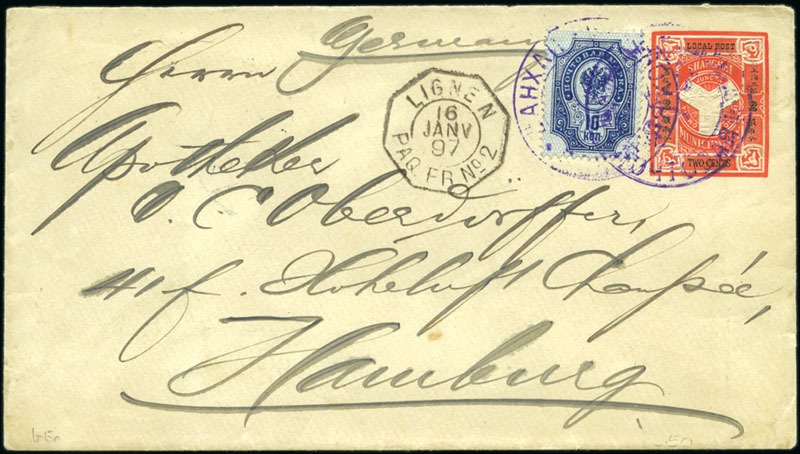
\includegraphics[width=.95\textwidth]{../russian-post-offices-in-china/10052.jpg}
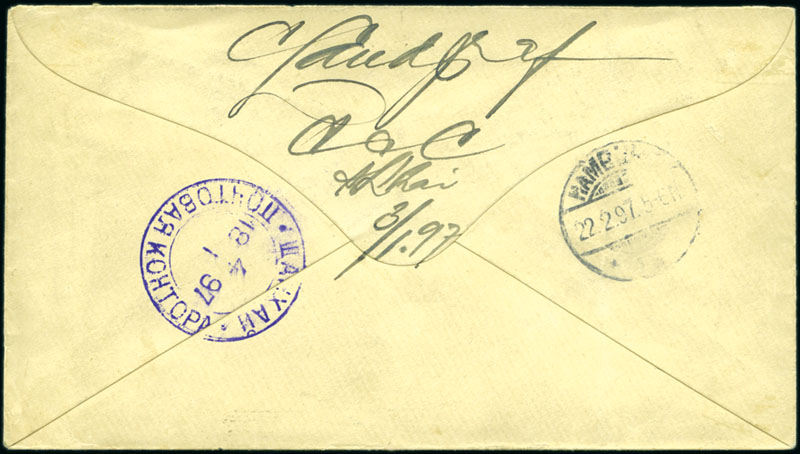
\includegraphics[width=.95\textwidth]{../russian-post-offices-in-china/10052-1.jpg}
\caption{
10052	SHANGHAI: 2c Shanghai Local Post embossed stationery envelope
with additional Russian 10k, the latter paying the single rate to
Germany and tied by Shanghai 4.1.97 cds in purple (T\&S type 1) with
further strike on reverse, with French paquebot ds ("Ligne N" 
Yokohama-Marseille No.2 on board SS "Tamise"), Hamburg bs.
The earliest known mail from the Russian P.O. in Shanghai
\euro 4,000.00. 
}  
\end{figure} 

\begin{figure}[htbp]
\centering
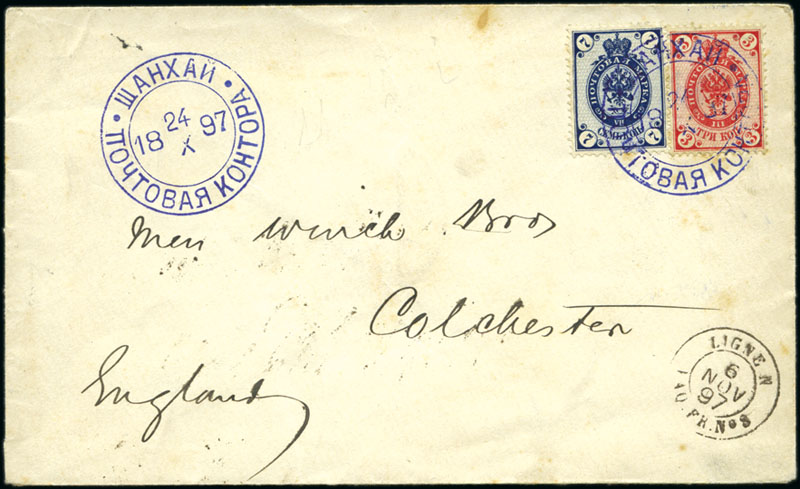
\includegraphics[width=.95\textwidth]{../russian-post-offices-in-china/10053.jpg}
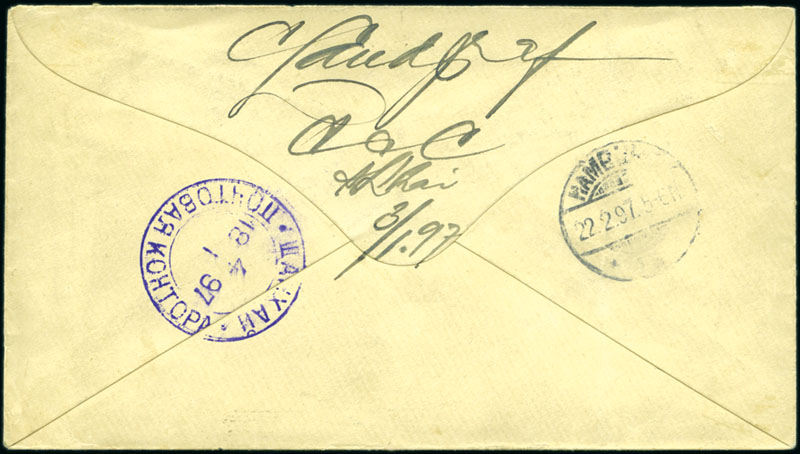
\includegraphics[width=.95\textwidth]{../russian-post-offices-in-china/10052-1.jpg}
\caption{
10053 SHANGHAI: 1897 Cover to England with Arms 7k and 3k 
tied by double ring Shanghai 24.10.97 cds in blue (T\&S type 1), 
with French paquebot ds adjacent, superb cancellation
\euro 500.00
}  
\end{figure} 

\begin{figure}[htbp]
\centering
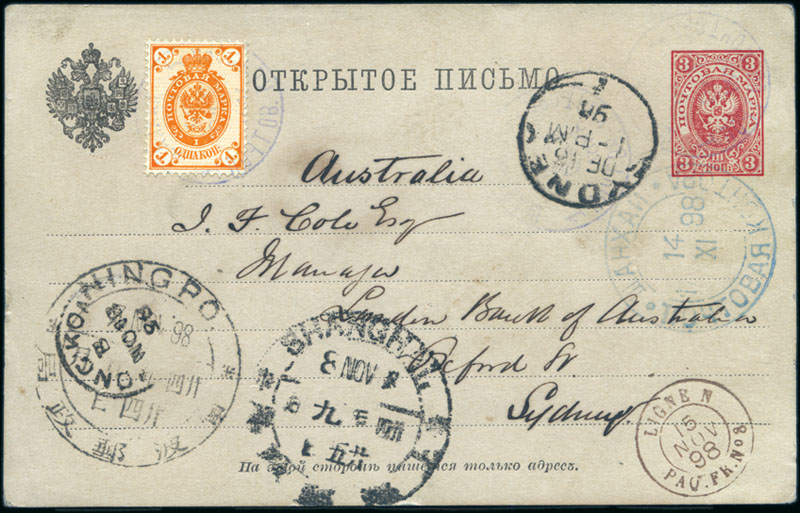
\includegraphics[width=.95\textwidth]{../russian-post-offices-in-china/10054.jpg}
\caption{
10054 SHANGHAI: 1898 3k Postcard uprated with Arms 1k from NINGPO to Australia, 
sent via Chinese Imperial Post to the Russian P.O. at Shanghai where it was 
cancelled with Shanghai 28.10.98 (9.11.98 in Gregorian calendar) cds in violet 
(T\&S type 2), with further Shanghai 14.11.98 (in Gregorian calendar)
cds in blue (T\&S type 1) before being sent by French paquebot to Hong Kong, 
then on to Sydney, all transits present, fine and very interesting card

Note: From Feb. 1897 the Chinese Imperial Post abolished the 
inland charge for carriage of foreign mail, with message on card 
confirming this fact: "Am writing this on a Russian card and posting 
it here in this city, if there is anything to pay on it, it will be an overcharge."
\euro 800.00. 
}  
\end{figure} 

\begin{figure}[htbp]
\centering
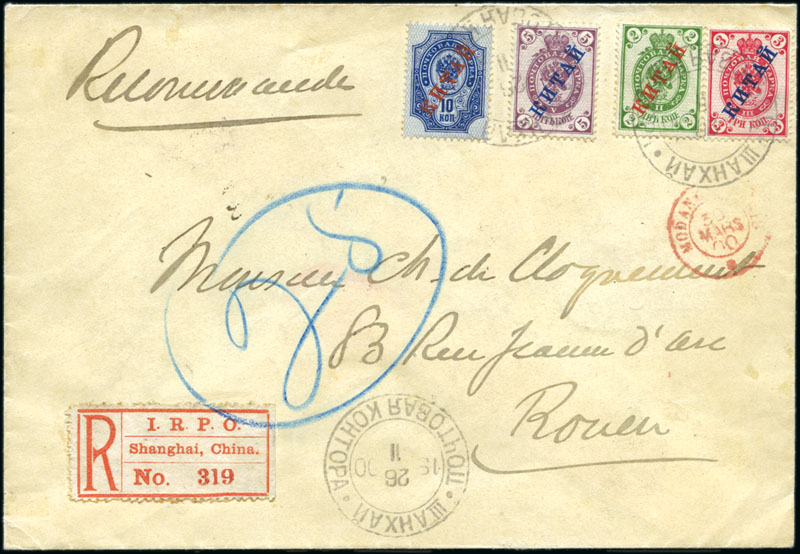
\includegraphics[width=.95\textwidth]{../russian-post-offices-in-china/10055.jpg}
\caption{
10055	SHANGHAI: 1900 Cover registered to France with "KITAI" 2k, 3k, 5k 
and 10k tied by Shanghai 26.2.1900 cds (T\&S type 1), with rare registration 
label in English at lower left reading "I(mperial). R(ussian). P(ost). O(ffice). / 
Shanghai, China," an attractive franking and rare registered cover
\euro 800.00 
}  
\end{figure} 














                                                                    